While first and second moments give us some idea of the performance of our sampling algorithms, we ideally would like a fuller picture.  In this section we compare the performance of algorithms using the total variation distance, $L^2$-Wasserstein distance and Kullback--Leibler divergence.  Using these measures, we can compare the performance to theoretical upper bounds for \texttt{ULA}.

\subsection{Statistical Distances}
Let $\mathcal{B}(\R^d)$ denote the Borel $\sigma$-algebra on $\R^d$. Let $P$ and $Q$ be probability measures on the space $(\R^d, \mathcal{B}(\R^d))$.  Then we define the total variation distance, Kullback--Leibler divergence and Wasserstein metric as follows:

\begin{defn}[Total Variation]
The total variation distance between two probability measures $P$ and $Q$ on $(\Omega, \mathcal{F})$ is defined as
$$
\norm{P - Q}_{TV} = \sup_{A \in \mathcal{F}} \abs{P(A) - Q(A)}.
$$
\end{defn}
\begin{prop}
If the set $\Omega$ is countable then this is equivalent to half the $L^1$ norm.
$$
\norm{P - Q}_{TV} = \frac{1}{2} \norm{P-Q}_1 = \frac{1}{2} \sum_{\omega \in \Omega} \abs{P(\omega) - Q(\omega)}
$$
\end{prop}
\begin{proof}
Let $B = \{\omega: P(\omega) \geq Q(\omega)\}$ and let $A \in \mathcal{F}$ be any event.  Then
$$
P(A) - Q(A) \leq P(A \cap B) - Q(A \cap B) \leq P(B) - Q(B).
$$
The first inequality holds since $P(\omega)-Q(\omega) < 0$ for any $\omega \in A \cap B^c$, and so the difference in probability cannot be greater if these elements are excluded.  For the second inequality, we observe that including further elements of $B$ cannot decrease the difference in probability.
Similarly,
$$
Q(A) - P(A) \leq Q(B^c) - P(B^c) = P(B) - Q(B)
$$
Thus, setting $A=B$, we have that $\abs{P(A)-Q(A)}$ is equal to the upper bound in the total variation distance.  Hence,
$$
\norm{P-Q}_{TV} = \frac{1}{2} \abs{P(B)-Q(B)+Q(B^c)-P(B^c)} = \frac{1}{2} \sum_{\omega \in \Omega} \abs{P(x)-Q(x)}
$$
\end{proof}


\textbf{POSSIBLY TAKE OUT KL DIVERGENCE??}

\begin{defn}[Kullback--Leibler Divergence]
Let $P$ and $Q$ be two probability measures on $(\Omega, \mathcal{F})$.  If $P \ll Q$, the Kullback--Leibler divergence of $P$ with respect to $Q$ is defined as
$$
KL(P|Q) = \int_\Omega \frac{d P}{d Q} log \left(  \frac{d P}{d Q} \right) d Q.
$$
\end{defn}

\textbf{LITTLE MORE INTUITION ON WASSERSTEIN \& TRANSPORT??}

Finally we consider the Wasserstein distance.  If $P$ and $Q$ are probability measures on $(\R^d,\mathcal{B}(\R^d)$, we say that $\gamma$ is a transport plan between two probability measures $P$ and $Q$ if it is a probability measure on $(\R^d \times \R^d, \mathcal{B}(\R^d \times \R^d))$ such that for any Borel set $A \subset \R^d$, $\gamma(A \times \R^d)=P(A)$ and $\gamma(\R^d \times A) = Q(A)$.  We denote the set of all such transport plans by $\Pi(P,Q)$.

\begin{defn}[Wasserstein distance]
For two probability measures, $P$ and $Q$, the $L^p$-Wasserstein distance is given by
$$
W_p(P,Q) = \left( \inf_{\gamma \in \Pi(P,Q)} \int_{\R^d \times \R^d} \norm{x-y}^p d \gamma(x,y) \right)^{1/p}.
$$
\end{defn}

We will restrict our attention mainly to $L^1$-Wasserstein and $L^2$-Wasserstein distances. Due to practical impossibility of computing higher-dimensional Wasserstein distances, we also introduce a compuatationally more feasible variant, the Sliced Wasserstein distance. First proposed in \cite{rabin2011wasserstein} and further elaborated on, for example, in \cite{gswd}, the Sliced Wasserstein distance exploits the fact that the Wasserstein distance between 1-dimensional probability measures $P, Q$ can be computed with an explicit formula $\abs{F^{-1}(t)-G^{-1}(t)}^p dt$ where $F$ and $G$ are the CDFs of $P$ and $Q$ respectively \cite{ramdas2017wasserstein}.


\begin{defn}[Sliced Wasserstein distance]
For two probability measures, $P$ and $Q$, the $L^p$-Wasserstein distance is given by
$$
SW_p(P,Q) = \left(\int_{\mathbb S^{d-1} }  W_p^p\left(\mathcal{RI}_P(\cdot, \theta), \mathcal{RI}_Q(\cdot, \theta) \right) d \theta \right)^{\frac 1 p}
$$
\end{defn}

where $\mathbb S^{d-1}$ is the $(d-1)$-dimensional sphere and $\mathcal RI$ denotes the Inverse Radon transform. In the above references, it is also proved that $SW_p$ is indeed a metric. The main reason why we can use the Sliced Wasserstein distance as an approximation to the Wasserstein distance is that these two metrics are equivalent\cite{Santa}.


\subsection{Theoretical Non-asymptotic Error Bounds}


Theoretical bounds on the total variation distance between the distribution of the $n^{\text{th}}$ iterate of the unadjusted Langevin Algorithm were first provided in the case of a `warm start' in \cite{dalalyan2017theoretical}. 

 Then \cite{durmus2016high}, \cite{durmus2017nonasymptotic} improve and consider Wasserstein distance.  These papers showed that $O(d/\epsilon)$ iterations are needed for precision level $\epsilon$.

\texttt{ULA} \cite{dalalyan2019user}
\texttt{tULA} \cite{Brosse18tULA}
\texttt{HOLA} \cite{Sabanis18tHOLA}
\texttt{MALA} \cite{bou2013nonasymptotic}



\section{Comparison of methods}
We have implemented a suite of tools for analysis of error for all of the aforementioned Langevin Monte Carlo algorithms. This section contains a selection of results, as well as a description of error metrics available and any other design choices made. The \textsc{Python} code and a how-to-use guide can be found at the following
\textsc{url}: \\

   \centerline{ \url{https://github.com/Tom271/LangevinMC}}


\subsection{Results}

\begin{figure}[H]
\centering
  \begin{minipage}[b]{0.49\textwidth}
  \centering
    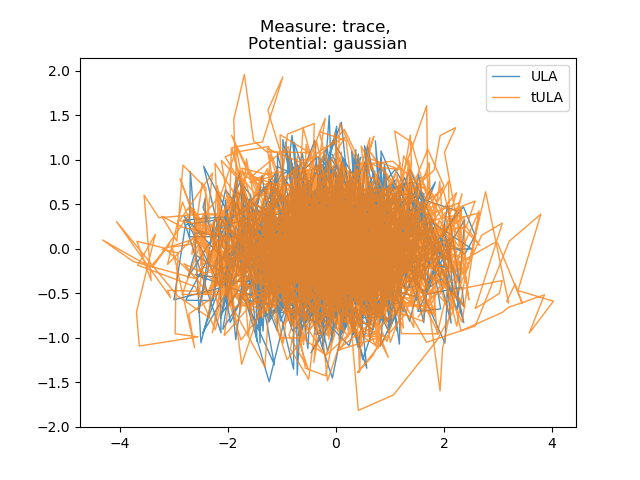
\includegraphics[width=\textwidth]{Figures/ula_tula_step_01.png}
  \end{minipage} %
  \begin{minipage}[b]{0.49\textwidth}
  \centering
    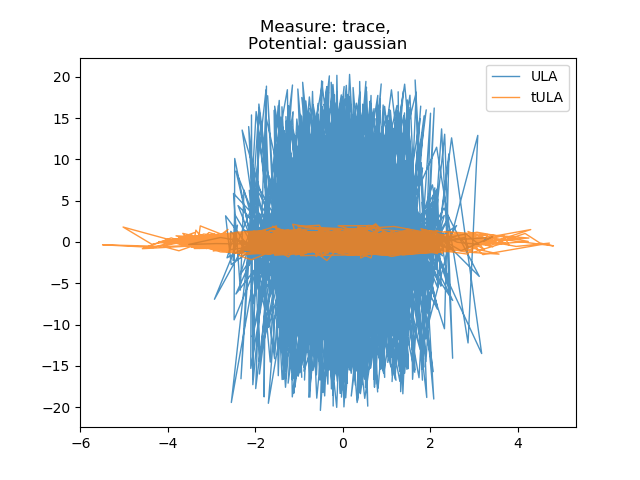
\includegraphics[width=\textwidth]{Figures/ula_tula_step_02.png}
  \end{minipage}
   \caption{\textbf{Demonstration of the stiffness problem with \texttt{ULA}}, resolved by taming. Both \texttt{ULA} and \texttt{tULA} work well for step size $h = 0.1$ on the left, however \texttt{ULA} becomes stiff for a larger step size $h = 0.2$ on the right. For ever higher step sizes, \texttt{ULA} diverges. The distribution here is Gaussian with covariance matrix $\text{diag}(1.0, 0.1)$.}
\end{figure}

\begin{figure}[H]
\centering
  \begin{minipage}[b]{0.49\textwidth}
  \centering
    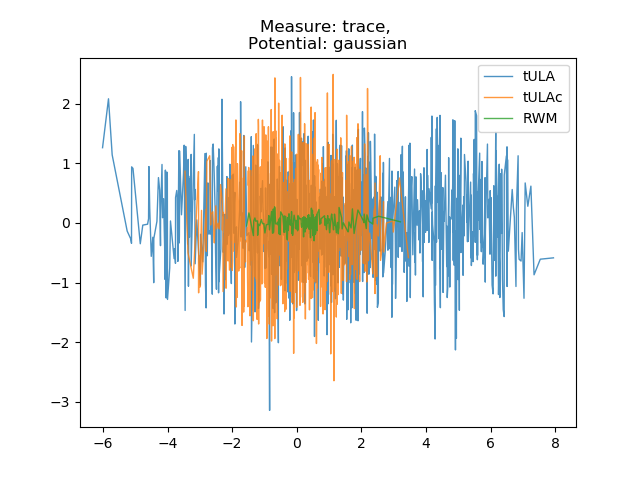
\includegraphics[width=\textwidth]{Figures/tula_tulac_rwm_stiff.png}
  \end{minipage} %
   \caption{\textbf{Coordinate-wise taming} can deal with stiffness in one axis (Ill-conditioned Gaussian distribution with covariance $\text{diag}(1.0, 0.01)$).}
\end{figure}



\begin{figure}[H]
\centering
  \begin{minipage}[b]{0.49\textwidth}
  \centering
    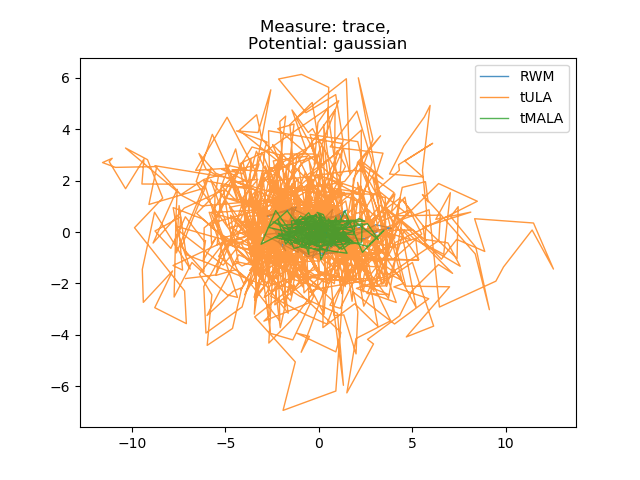
\includegraphics[width=\textwidth]{Figures/tula_tmala_step_1.png}
  \end{minipage} %
  \begin{minipage}[b]{0.49\textwidth}
  \centering
    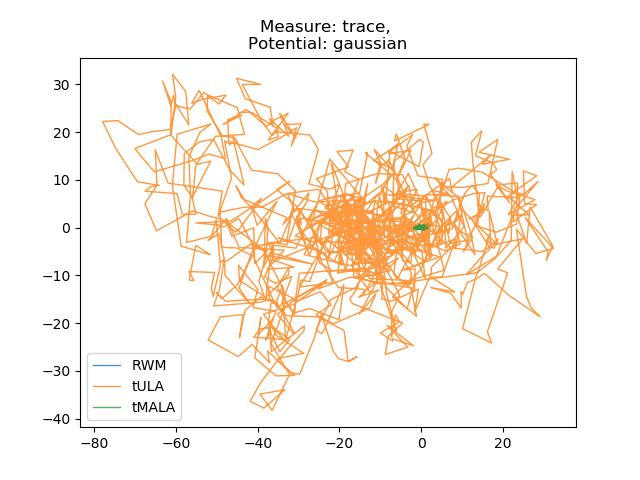
\includegraphics[width=\textwidth]{Figures/tula_tmala_step_10.png}
  \end{minipage}
   \caption{\textbf{Trade-off between rejection-based algorithms and \texttt{tULA} for large step-sizes} ($h = 1$ on the left and $h = 10$ on the right, distribution is Gaussian with covariance matrix $\text{diag}(1.0, 0.1)$). With increasing step size, even \texttt{tULA} starts to suffer from stiffness problems. Rejection-based algorithms resolve the issue, however, their acceptance rate drops very low ($\approx 0.2$ on the left and $\approx 0.03$ on the right). }
\end{figure}



\begin{figure}[H]
\centering
  \begin{minipage}[b]{0.32\textwidth}
  \centering
    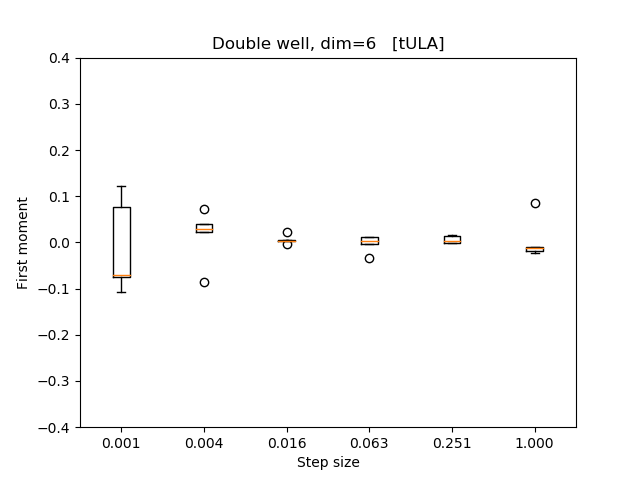
\includegraphics[width=\textwidth]{Figures/tula_fm.png}
  \end{minipage} %
  \begin{minipage}[b]{0.32\textwidth}
  \centering
    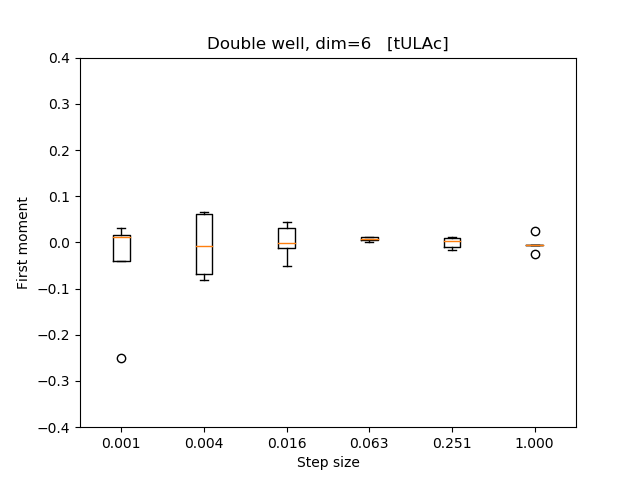
\includegraphics[width=\textwidth]{Figures/tulac_fm.png}
  \end{minipage} %
  \begin{minipage}[b]{0.32\textwidth}
  \centering
    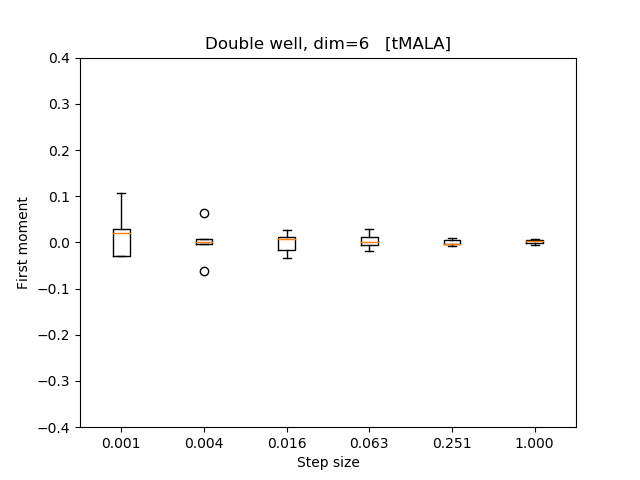
\includegraphics[width=\textwidth]{Figures/tmala_fm.png}
  \end{minipage}
   \caption{Comparison of \texttt{tULA}, \texttt{tULAc} and \texttt{tMALA} for the first moment evolving as a function of step size.}
\end{figure}


\begin{figure}[H]
\centering
  \begin{minipage}[b]{0.32\textwidth}
  \centering
    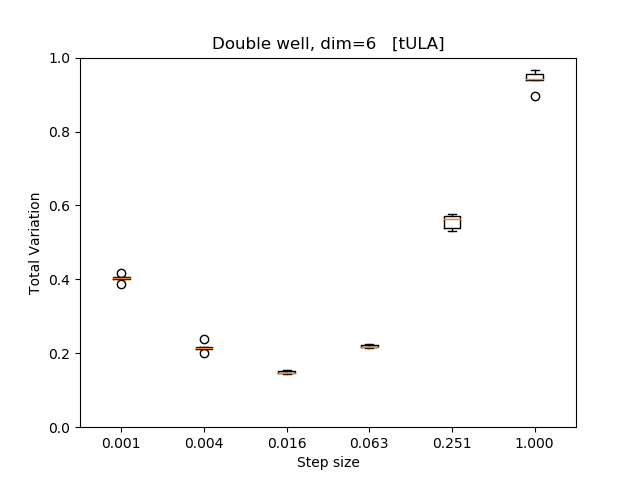
\includegraphics[width=\textwidth]{Figures/tula_tv.png}
  \end{minipage} %
  \begin{minipage}[b]{0.32\textwidth}
  \centering
    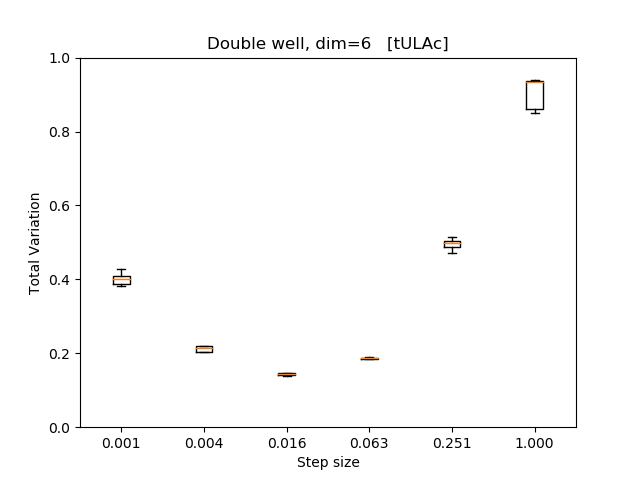
\includegraphics[width=\textwidth]{Figures/tulac_tv.png}
  \end{minipage} %
  \begin{minipage}[b]{0.32\textwidth}
  \centering
    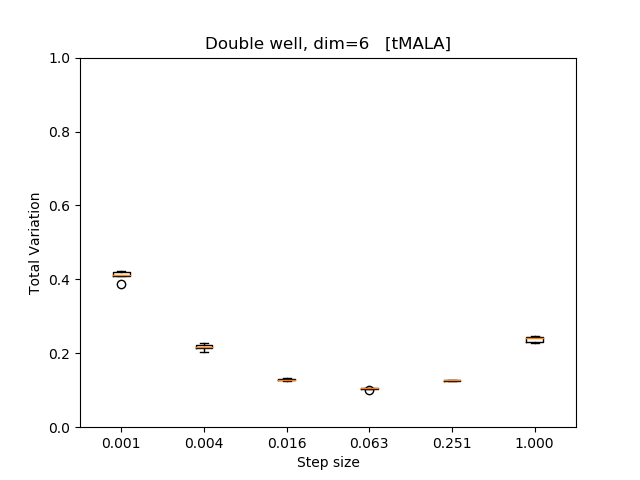
\includegraphics[width=\textwidth]{Figures/tmala_tv.png}
  \end{minipage}
   \caption{Comparison of \texttt{tULA}, \texttt{tULAc} and \texttt{tMALA} for the total variation error evolving as a function of step size.}
\end{figure}




\subsection{Sampling approaches}

Our program allows to specify

In general, there are two main approaches to sampling

\subsection{Parameters}






\subsection{Estimating error}

In the following, let $\pi$ be the pdf of true distribution from which we attempt to sample and $X = \{x_i\}_{i=1}^N$ denote the collection of samples collected by a sampling algorithm. The notation $x_i(d)$ will be used to refer to the $d$-th coordinate of $x_i$. We also denote by $\{m_d\}_{d=1}^D$ and $\{M_d\}_{d=1}^D$ the coordinate-wise minimums and maximums among $x_i$, that is:

$$ 
    m_d = \min \{x_i(d)\}_{i=1}^N \ \ \text{ and } \ \ M_d = \max \{x_i(d)\}_{i=1}^N
$$

For some of the error estimation methods, it will be necessary to construct multi-dimensional histograms. For this purpose, we define the following set of points (this is a minimal mesh that spans all of the samples):

$$
\#_X := \left\{ \left(c_1^{(k_1)}, c_2^{(k_2)}, \dots, c_D^{(k_D)}\right)\ |\ (k_1, k_2, \dots, k_D) \in \{0, 1, \dots, \text{bins - 1}\}^D, \ c_d^{(k_d)} = m_d + \left(k_d + \frac 1 2\right) \frac{M_d - m_d}{\text{bins}} \right\}
$$

where $bins$ is a parameter describing the fineness of the mesh. The histogram of the collection of samples $X$ will be understood to be the following function $h: \#_X \rightarrow \mathbb R$:

$$
    h(c) = \frac 1 N |\{x \in X\ |\ \arg \min_{c' \in \#_X} \norm{c' - x} = c \}|
$$

i. e. normalized count of points $x$ such that the closes point of mesh to $x$ is $c$. This defines the discrete probability measure 

$$H_X := \sum_{c \in \#_X} h(c) \delta_c,$$

which we will understand to be the sampled approximation of the true distribution from which we are sampling. Finally, denote also by $Z$ the sum of the true distribution pdf values over the values of the mesh.

\[Z := \sum_{c \in \#_X} \pi(c)\]

\begin{itemize}
    \item sliced W
    \item sliced W no histo
    \item KDE KL, TV, SW
\end{itemize}



\subsubsection{Comparing continuous and discrete distributions: histograms vs. KDE}


\subsubsection{The Curse of dimensionality}

In short, since $|\#_X| = \text{bins}^D$ is exponential in dimension, it is impossible to construct histograms in high dimensions.

\subsection{Implemented metrics}

\subsubsection{Visualizations}
In special cases when the dimension is $1$ or $2$, we have implemented an option to visualize the samples either as a histogram plot (in 1D) or as a scatter or trace plot (in 2D or 3D).


\begin{figure}[H]
\centering
  \begin{minipage}[b]{0.3\textwidth}
  \centering
    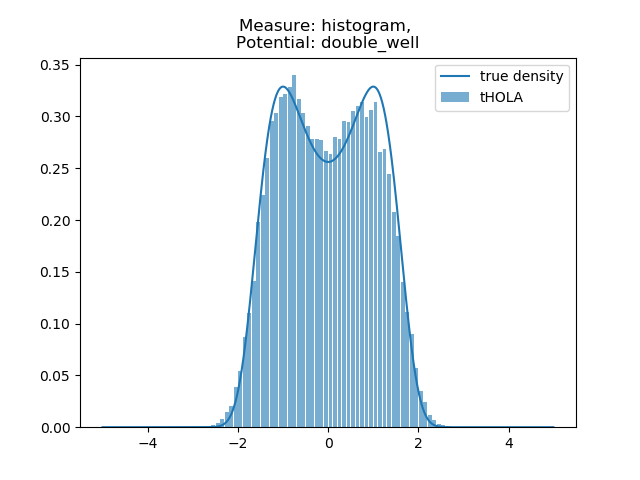
\includegraphics[width=\textwidth]{Figures/histo_example.png}
  \end{minipage} %
  \begin{minipage}[b]{0.3\textwidth}
  \centering
    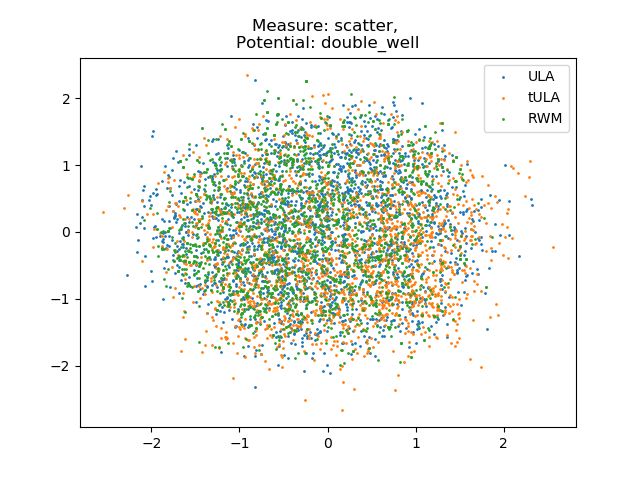
\includegraphics[width=\textwidth]{Figures/scatter_example.png}
  \end{minipage} %
  \begin{minipage}[b]{0.3\textwidth}
  \centering
    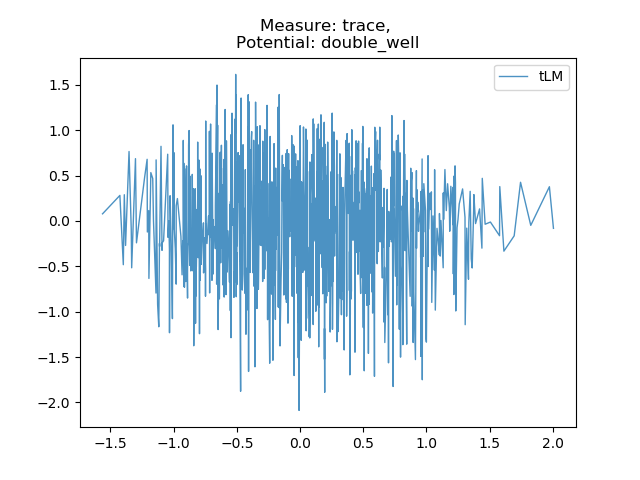
\includegraphics[width=\textwidth]{Figures/trace_example.png}
  \end{minipage}
   \caption{Example of a histogram plot, scatter plot and a trace plot.}
\end{figure}



\subsubsection{First/Second moments}
The first and second moments are implemented in the standard way. By default, the result is computed \textit{in the first coordinate only\footnote{With option to use $\frac 1 N\sum_{i=1}^N \norm{x_i}$ and $\frac 1 N\sum_{i=1}^N \norm{x_i^2}$ instead.}}.

$$ 
    \text{first moment} = \frac 1 N\sum_{i=1}^N x_i(1) \qquad \text{ and } \qquad \text{second moment} = \frac 1 N\sum_{i=1}^N x_i(1)^2
$$


\subsubsection{Total variation}
The total variation, being the first of implemented histogram measures, is calculated as

\[\text{total variation} = \norm{H_X - \frac 1 Z \sum_{c \in \#_X} \pi(c) \delta_c}_{\text{TV}} = \frac 1 2\sum_{c \in \#_X} \left|\frac{h(c)}{N} - \frac{\pi(c)}{Z}\right| .\]

\subsubsection{KL Divergence}
The next histogram-based measure is KL divergence.

\[\text{KL divergence} = \text{KL} \left(H_X \bigg| \frac 1 Z \sum_{c \in \#_X} \pi(c) \delta_c\right) =  \sum_{c \in \#_X} \frac{h(c)}{N} \log\left(\frac {h(c) Z} {\pi(c) N} \right).\]

\subsubsection{Sliced Wasserstein}

The Sliced Wasserstein distance, being defined via a multi-dimensional integral, cannot be computed exactly. Therefore, we resort to a simple Monte Carlo scheme where $L$ samples $\{\theta_i\}$ are drawn uniformly from the $(d-1)$-dimensional sphere $\mathbb S^{d-1}$.

$$ 
SW_p(P, Q) \approx \left( \frac 1 L \sum_{i=1}^L W_p^p\left(\mathcal{RI}_P(\cdot, \theta_i), \mathcal{RI}_Q(\cdot, \theta_i) \right) \right)^{\frac 1 p}
$$

The first, histogram based, implemented metric for Sliced Wasserstein distance further approximates the above Monte Carlo scheme for $SW_1\left(H_X, \right)$ as

\[\text{SW}_{histogram} = \begin{cases}
W_1 \left( H_X,\  \frac 1 Z \sum_{c \in \#_X} \pi(c) \delta_c \right) & \text{if dimension } = 1 \\
\sum_{i = 1}^L W_1 \left( \sum_{c \in \#_X} h(c) \delta_{\left<c, \theta_i \right>},\  \frac 1 Z \sum_{c \in \#_X} \pi(c) \delta_{\left<c, \theta_i \right>}  \right) & \text{ otherwise }
\end{cases},\]

where $\left< \cdot \right>$ is the dot product, $\theta_i = \frac{\theta'_i}{\norm{\theta'_i}}$ is a point on $(d-1)$-dimensional sphere with $
\theta'_i \sim \mathcal N(0, I_D)$ and $W_1$ is computed explicitly. \\\\

The second, \textbf{heuristic-based}, approximation of the Sliced Wasserstein distance is calculated as follows:

\[\text{SW}_{no\ histogram} = \begin{cases}
W_1 \left( \frac 1 N \sum_{x \in X} \delta_x,\  \frac 1 {Z'} \sum_{x \in X} \pi(x) \delta_x \right) & \text{if dimension } = 1 \\
\sum_{i = 1}^L W_1 \left(  \frac 1 N \sum_{x \in X} \delta_{\left<x, \theta_i \right>},\ \frac 1 {Z'} \sum_{x \in X} \pi(x) \delta_{\left<x, \theta_i \right>}  \right) & \text{ otherwise }
\end{cases}.\]
where $Z' = \sum_{x \in X} \pi(x) $ is a normalizing constant. Intuitivelly, this measure of error describes whether the spatial distribution of samples is proportional to the true distribution, \textit{at the same points}.


\subsection{KDE-based metrics}